\documentclass{exam}

\usepackage{units} 
\usepackage{xfrac} 
\usepackage[fleqn]{amsmath}
\usepackage{cancel}
\usepackage{float}
\usepackage{mdwlist}
\usepackage{booktabs}
\usepackage{cancel}
\usepackage{polynom}
\usepackage{caption}
\usepackage{fullpage}
\usepackage{comment}
\usepackage{enumerate}
\usepackage{graphicx}

\newcommand{\degree}{\ensuremath{^\circ}} 
\everymath{\displaystyle}

\printanswers

\ifprintanswers 
  \usepackage{2in1, lscape} 
\fi

\author{}
\date{January 29, 2014}
\title{Statistics \\ Homework One}

\begin{document}

  \maketitle

  \begin{itemize*}
    \item read Chapter 2 
    \item answer the questions in ``Check Your Skills'' and check the answers in the back of the book
    \item hand in exercises TO DO
  \end{itemize*}

  \ifprintanswers
    \begin{description}
      \item[25] The larger number is the mean because the mean is dragged upward by a few people who make hundreds of
        thousands of dollars.

      \item[26] For the people who are still working (21-64), there are a lot of young people with almost no retirement
        money and a few older people with large retirement accounts.  This makes the distribution right-skewed and the
        mean is larger than the median.

        For the people who are mostly retired (55 or older), almost everyone has some retirement money saved, and there
        are only a few people with no retirement money.  This makes the distribution left-skewed and the mean is smaller
        than the median.

      \item[27] 
        \begin{itemize*}
          \item the median is college 393
          \item the first quartile is college 197
          \item the third quartile is college 590
        \end{itemize*}

      \item[29]
        \begin{figure}[H]
          \centering
          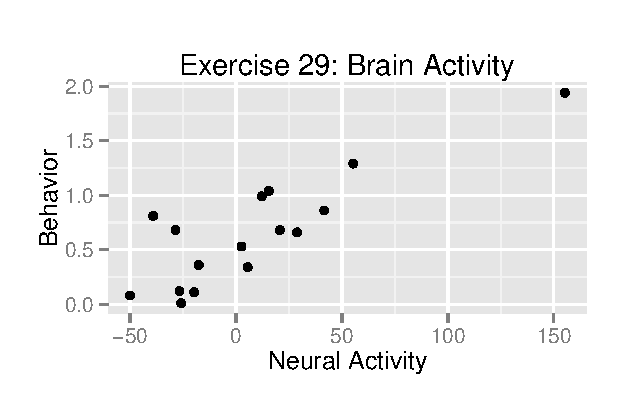
\includegraphics{figures/ex29.eps}
          \caption{Exercise 29}
        \end{figure}

        \begin{table}[ht]
          \centering
          \begin{tabular}{rlrrrrrr}
            \toprule
              & Variety & Min.  & 1st Qu. & Median & Mean  & 3rd Qu. & Max. \\
            \midrule
            1 & bihai   & 46.34 & 46.73   & 47.12  & 47.60 & 48.20   & 50.26 \\
            2 & red     & 37.40 & 38.08   & 39.16  & 39.71 & 41.58   & 43.09 \\
            3 & yellow  & 34.57 & 35.56   & 36.11  & 36.18 & 36.80   & 38.13 \\
            \bottomrule
          \end{tabular}
        \end{table}

        The summary doesn't show the shape that the histogram does.

      \item[30]
        If you add up all the bars, you find that there are 78 girls.  The median would be between girl number 39 and
        40, which would be in the 2 servings bar.  The first quartile would be girl 19 which is in the 1 serving bar and
        the third quartile would be girl 59 which is in the 4 servings bar.  So the answer is:

        \begin{itemize*}
          \item first quartile: 1
          \item median: 2
          \item third quartile: 4
        \end{itemize*}
        
      \item[32]
        \begin{parts}
          \part symmetric distributions without outliers

          \part 
            \begin{itemize*}
              \item for the men, $\bar{x}$ went from 117.17 to 110.86 and $s$ went from 74.24 to 66.88
              \item for the women, $\bar{x}$ went from 165.17 to 158.45 and $s$ went from 56.51 to 43.65
            \end{itemize*}

        \end{parts}

    \end{description}

  \else
    \vspace{11 cm}
    \begin{quote}
      \begin{em}
        Even voting for the right is doing nothing for it. It is only expressing to men feebly your desire that it
        should prevail. 
        % A wise man will not leave the right to the mercy of chance, nor wish it to prevail through the power of the
        % majority. There is but little virtue in the action of masses of men. When the majority shall at length vote for
        % the abolition of slavery, it will be because they are indifferent to slavery, or because there is but little
        % slavery left to be abolished by their vote. 
      \end{em}
    \end{quote}
    \hspace{1 cm} --Henry David Thoreau
  \fi

\end{document}

